\documentclass{article}
\usepackage[a4paper]{geometry}
\usepackage{amsfonts}
\usepackage{alltt}
\usepackage{amsmath,amssymb}        % Mathpack für Formeln jeder Art
\usepackage[parfill]{parskip}       % Autoamtisch Newline, wenn Zeilenumbruch im Quelltext.
\usepackage[utf8]{inputenc}         % UTF8 Zeichensatz. 
\usepackage{xstring}				% Gebraucht für Circuitikz
\usepackage{tikz}                   % Wichtig für Zeichnungen aller Art
\input{kvmacros}                    % Kv Diagramme
\usepackage[siunitx]{circuitikz}    % Diagramme und Schaltungen
\usepackage{pgffor}					
\usepackage{fancyhdr}				
\usepackage{array}		


\tikzstyle{n}=[fill,circle,radius=0.4cm,font=\huge,inner sep=0,minimum size=0.5em]


\title{Mathematik Hausaufgaben zum 14. Dezember}
\author{Arne Beer, MN 6489196 \\
 Tim Overath, MN 6440863\\
 Paul Bienkowski}

\begin{document}
\maketitle

\section*{Aufgabe 1}
	
	\subsection*{a)}
		Bei den beiden abgebildeten Graphen besteht kein Isomorphismus, da sich bei dem 1. Graph sechs 4-Kreise und beim 2. Graph sieben 4-Kreise bilden lassen

	\subsection*{b)}

		Der erste und der dritte Graph sind isomoerph zueinander

\section*{Aufgabe 2}
	\subsection*{a)}
		$\frac{10\cdot 9}{2}=45$ Kanten

	\subsection*{b)}
		$\binom{10}{3}=120$ Kreise der Länge 3

	\subsection*{c)}
		$\binom{10}{4}=210$ Kreise der Länge 3


	\subsection*{d)}
		Da jeder Knoten mit jedem anderen Knoten verbunden ist, entsteht der
		Graph H bei allen zufällig herausgegriffenen 4 Knoten. Es gibt dann aber bei
		solch einer Auswahl von 4 Knoten zwei Möglichkeiten, sie zu H anzuordnen.
		Also ist die Menge der Teilgraphen, isomorph zum abgebildeten Graphen H sind:
		\[\binom{10}{4}\cdot 2 = 420\]

\section*{Aufgabe 1}
	\subsection*{a)}
	n=4 \\
	\\
	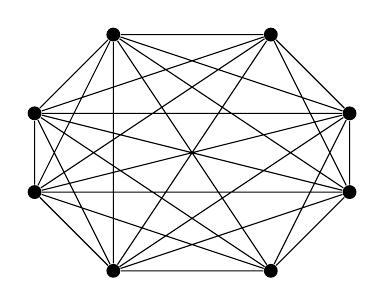
\begin{tikzpicture}
	 
                        \node[n] (a) at (1, 0) {};
                        \node[n] (b) at (0, 1) {};
                        \node[n] (c) at (0, 2) {};
                        \node[n] (d) at (1, 3) {};

                        \node[n] (e) at (3, 0) {};
                        \node[n] (f) at (4, 1) {};
                        \node[n] (g) at (4, 2) {};
                        \node[n] (h) at (3, 3) {};

                        \draw
                        (a) -- (b)
                        (b) -- (c)
                        (c) -- (d)
                        (d) -- (h)
                        (e) -- (f)
                        (f) -- (g)
                        (g) -- (h)
                        (a) -- (e)

                        (a) -- (c)
                        (a) -- (d)
                        (a) -- (f)
                        (a) -- (g)
                        (a) -- (h)

                        (b) -- (d)
                        (b) -- (e)
                        (b) -- (f)
                        (b) -- (g)
                        (b) -- (h)

                        (c) -- (e)
                        (c) -- (f)
                        (c) -- (g)
                        (c) -- (h)

                        (d) -- (e)
                        (d) -- (f)
                        (d) -- (g)
                        (d) -- (h)

                        (e) -- (f)
                        (e) -- (g)
                        (e) -- (g)

                        (f) -- (h)
                        (f) -- (a)

                        ;

    \end{tikzpicture}

   n=6\\
   \\
   	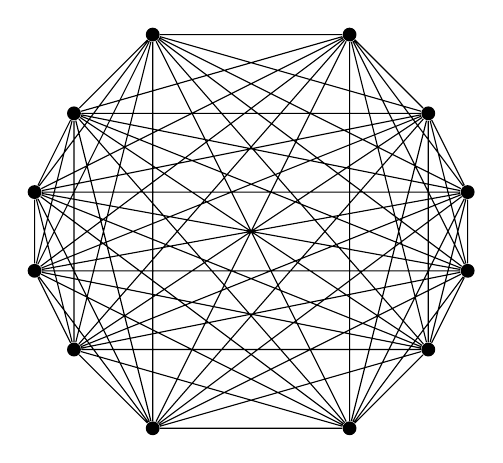
\begin{tikzpicture}
	 
                        \node[n] (a) at (1.5,0) {};
                        \node[n] (b) at (0.5,1) {};
                        \node[n] (c) at (0,2) {};
                        \node[n] (d) at (0,3) {};
                        \node[n] (e) at (0.5,4) {};
                        \node[n] (f) at (1.5,5) {};

                        \node[n] (g) at (4,0) {};
                        \node[n] (h) at (5,1) {};
                        \node[n] (i) at (5.5,2) {};
                        \node[n] (j) at (5.5,3) {};
                        \node[n] (k) at (5,4) {};
                        \node[n] (l) at (4,5) {};

                        \draw 
                        (a) -- (b)
                        (b) -- (c)
                        (c) -- (d)
                        (d) -- (e)
                        (e) -- (f)
                        (f) -- (l)
                        (g) -- (h)
                        (h) -- (i)
                        (i) -- (j)
                        (j) -- (k)
                        (k) -- (l)
                        (a) -- (g)

                        (a) -- (c)
                        (a) -- (d)
                        (a) -- (e)
                        (a) -- (f)
                        (a) -- (g)
                        (a) -- (h)
                        (a) -- (i)
                        (a) -- (j)
                        (a) -- (k)
                        (a) -- (l)

                        (b) -- (d)
                        (b) -- (e)
                        (b) -- (f)
                        (b) -- (g)
                        (b) -- (h)
                        (b) -- (i)
                        (b) -- (j)
                        (b) -- (k)
                        (b) -- (l)

                        (c) -- (e)
                        (c) -- (f)
                        (c) -- (g)
                        (c) -- (h)
                        (c) -- (i)
                        (c) -- (j)
                        (c) -- (k)
                        (c) -- (l)

                        (d) -- (f)
                        (d) -- (g)
                        (d) -- (h)
                        (d) -- (i)
                        (d) -- (j)
                        (d) -- (k)
                        (d) -- (l)

                        (e) -- (g)
                        (e) -- (h)
                        (e) -- (i)
                        (e) -- (j)
                        (e) -- (k)
                        (e) -- (l)

                        (f) -- (g)
                        (f) -- (h)
                        (f) -- (i)
                        (f) -- (j)
                        (f) -- (k)
                        (f) -- (l)
                        
                        (g) -- (i)
                        (g) -- (j)
                        (g) -- (k)
                        (g) -- (l)

                        (h) -- (j)
                        (h) -- (k)
                        (h) -- (l)

                        (i) -- (k)
                        (i) -- (l)
                        
                        (j) -- (l)
                        ;


    \end{tikzpicture}


	\subsection*{b)}
	Zwischen $H_1$ und $H_2:n^2$ Kanten
	$H_1$ besitzt $\frac{3\cdot n}{2}$
	$H_2$ besitzt $\frac {n \cdot (n-1)}{2}$
	Also ist die Gesamtkantenanzahl G:\\
	\[G= n^2 + \frac{3\cdot n}{2}+\frac{n\cdot (n-1)}{2}\]\\
	\[G=\frac{2n^2+3n+n^2-n}{2}\] \\
	\[G=\frac{3}{2}n^2+n\]\\

	\subsection*{c)}

	n=4 \\
	\\
	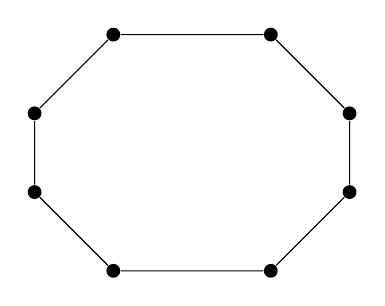
\begin{tikzpicture}
	 
                        \node[n] (a) at (1, 0) {};
                        \node[n] (b) at (0, 1) {};
                        \node[n] (c) at (0, 2) {};
                        \node[n] (d) at (1, 3) {};

                        \node[n] (e) at (3, 0) {};
                        \node[n] (f) at (4, 1) {};
                        \node[n] (g) at (4, 2) {};
                        \node[n] (h) at (3, 3) {};

                        \draw
                        (a) -- (b)
                        (b) -- (c)
                        (c) -- (d)
                        (d) -- (h)
                        (e) -- (f)
                        (f) -- (g)
                        (g) -- (h)
                        (a) -- (e)

                        ;

    \end{tikzpicture}

   n=6\\
   \\
   	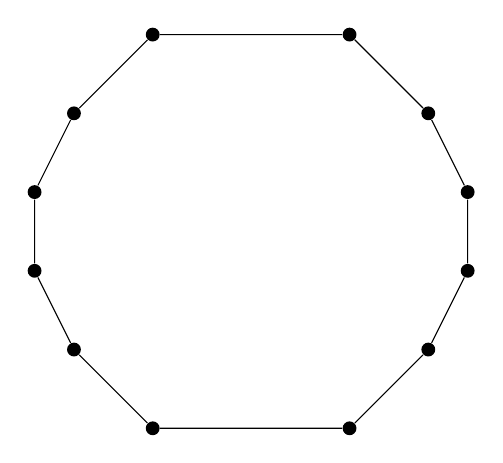
\begin{tikzpicture}
	 
                        \node[n] (a) at (1.5,0) {};
                        \node[n] (b) at (0.5,1) {};
                        \node[n] (c) at (0,2) {};
                        \node[n] (d) at (0,3) {};
                        \node[n] (e) at (0.5,4) {};
                        \node[n] (f) at (1.5,5) {};

                        \node[n] (g) at (4,0) {};
                        \node[n] (h) at (5,1) {};
                        \node[n] (i) at (5.5,2) {};
                        \node[n] (j) at (5.5,3) {};
                        \node[n] (k) at (5,4) {};
                        \node[n] (l) at (4,5) {};

                        \draw 
                        (a) -- (b)
                        (b) -- (c)
                        (c) -- (d)
                        (d) -- (e)
                        (e) -- (f)
                        (f) -- (l)
                        (g) -- (h)
                        (h) -- (i)
                        (i) -- (j)
                        (j) -- (k)
                        (k) -- (l)
                        (a) -- (g)
                        ;


    \end{tikzpicture}


	\subsection*{d)}

	Damit ein Graph eine Eulersche Linie hat, muss jeder Knoten einen geraden
	Grad haben.
	Alle Knoten von H1 haben den Grad 3 + n, weil von jedem Knoten, der
	sowieso schon den Grad 3 hat, noch einmal zu jedem Knoten von $H_2$ eineKante besitzt. Da n gerade ist, ist der Gesamtgrad jedes Knotens von $H_1$
	ungerade. Es gibt also auf keinen Fall eine Eulersche Linie.

\section*{Aufgabe 1}
	\subsection*{a)}

	\[|P(M)|=2^4=16\]

	\[ P(M)=\{\emptyset, \{a\},\{b\},\{c\},\{d\},\{a,b\},\{a,c\},\{a,d\},\{b,c\},\{b,d\},\{c,d\}\{a,b,c\},\{b,c,d\},\{a,b,d\},\{a,c,d\},\{a,b,c,d\}\} \]

	
	\subsection*{b)}
	   	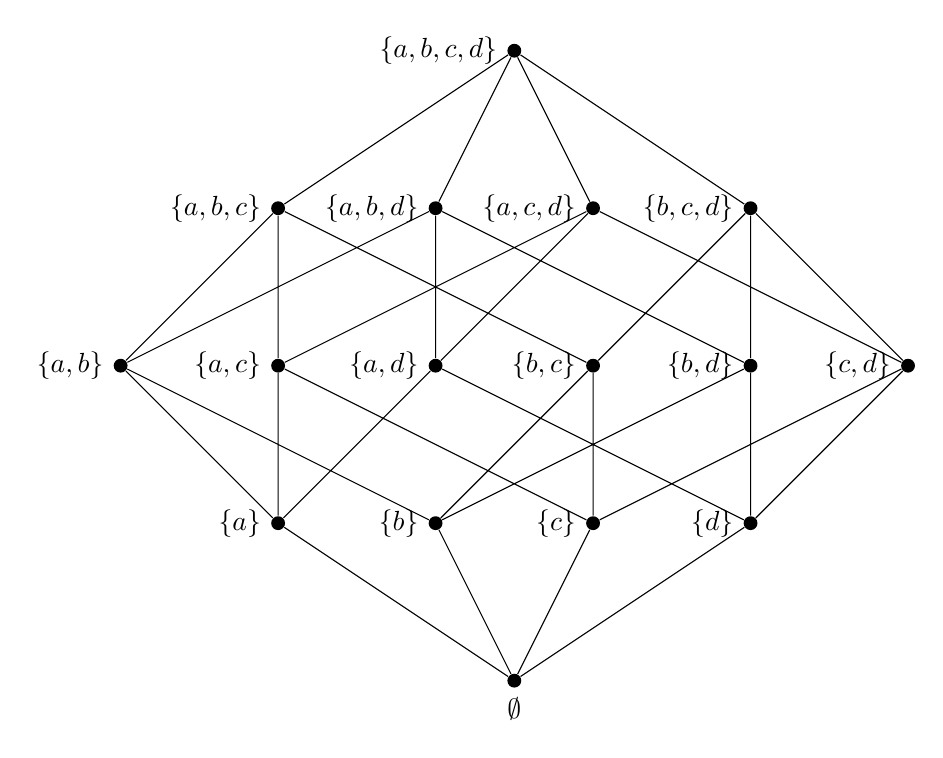
\begin{tikzpicture}
 						\node[n, label=below:$\emptyset$] (a) at (6,0) {};

                        \node[n, label=left:$\{a\}$] (b) at (3,2) {};
                        \node[n, label=left:$\{b\}$] (c) at (5,2) {};
                        \node[n, label=left:$\{c\}$] (d) at (7,2) {};
                        \node[n, label=left:$\{d\}$] (e) at (9,2) {};

                        \node[n, label=left:{$\{a,b\}$}] (f) at (1,4) {};
                        \node[n, label=left:{$\{a,c\}$}] (g) at (3,4) {};
                        \node[n, label=left:{$\{a,d\}$}] (h) at (5,4) {};
                        \node[n, label=left:{$\{b,c\}$}] (i) at (7,4) {};
                        \node[n, label=left:{$\{b,d\}$}] (j) at (9,4) {};
                        \node[n, label=left:{$\{c,d\}$}] (k) at (11,4) {};

                        \node[n, label=left:{$\{a,b,c\}$}] (l) at (3,6) {};
                        \node[n, label=left:{$\{a,b,d\}$}] (m) at (5,6) {};
                        \node[n, label=left:{$\{a,c,d\}$}] (n) at (7,6) {};
                        \node[n, label=left:{$\{b,c,d\}$}] (o) at (9,6) {};

                        \node[n,label=left:{$\{a,b,c,d\}$}] (p) at (6,8) {};

                        \draw

                        (a) -- (b)
                        (a) -- (c)
                        (a) -- (d)
                        (a) -- (e)

                        (b) -- (f)
                        (b) -- (g)
                        (b) -- (h)
                        
                        (d) -- (g)
                        (d) -- (i)
                        (d) -- (k)

                        (e) -- (h)
                        (e) -- (k)
                        (e) -- (j)

                        (c) -- (f)
                        (c) -- (i)
                        (c) -- (j)

                        (f) -- (l)
                        (f) -- (m)

                        (g) -- (l)
                        (g) -- (n)

                        (h) -- (m)
                        (h) -- (n)

                        (i) -- (l)
                        (i) -- (o)

                        (j) -- (o)
                        (j) -- (m)

                        (k) -- (o)
                        (k) -- (n)

                        (l) -- (p)
                        (m) -- (p)
                        (n) -- (p)
                        (o) -- (p)
                        ;

   		\end{tikzpicture}
	\subsection*{c)}

	Der Graph ist isomorph zum Graph aus der Präsenzaufgabe 2 a). Hierbei
	beschreibt eine 1, dass sich das Element in der Teilmenge befindet. So ist
	zum Beispiel das Tupel $(0, 0, 0, 0)$ die Darstellung der leeren Menge $\emptyset$ und
	$(1, 0, 0, 0)$ die Repräsentation der Teilmenge {a}.

\end{document}